\usetikzlibrary{calc}
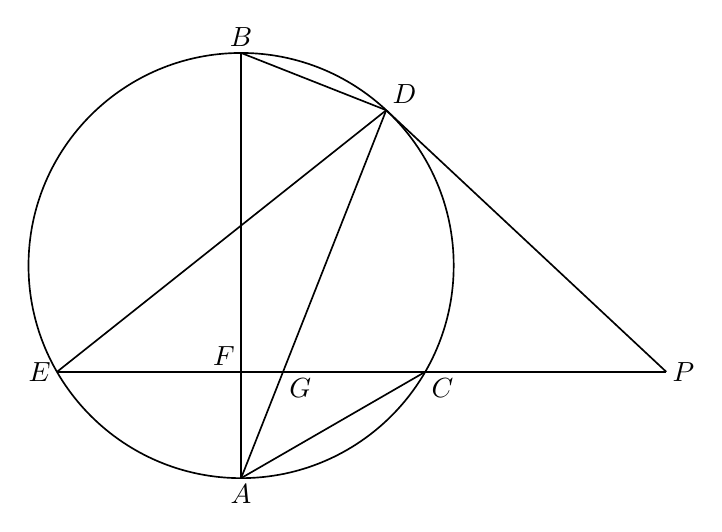
\begin{tikzpicture}[x=1cm,y=1cm,line width=.6pt,font=\normalsize]
\coordinate (Oaux) at (0,0);
\coordinate (E) at (-2.338269,-1.35);
\coordinate (C) at (2.338269,-1.35);
\coordinate (F) at (0,-1.35);
\coordinate (G) at (0.532506,-1.35);
\coordinate (A) at (0,-2.7);
\coordinate (B) at (0,2.7);
\coordinate (D) at (1.843235,1.972938);
\coordinate (P) at (5.4,-1.35);
\draw[black] (Oaux) circle[radius=2.7cm];
\draw[black] (E)--(P);
\draw[black] (A)--(B);
\draw[black] (E)--(D);
\draw[black] (A)--(D);
\draw[black] (A)--(C);
\draw[black] (B)--(D);
\draw[black] (D)--(P);
\node[left=2pt,inner sep=0pt] at (E) {$E$};
\node[above left=2pt,inner sep=0pt] at (F) {$F$};
\node[below right=2pt,inner sep=0pt] at (G) {$G$};
\node[below right=2pt,inner sep=0pt] at (C) {$C$};
\node[below=2pt,inner sep=0pt] at (A) {$A$};
\node[above=2pt,inner sep=0pt] at (B) {$B$};
\node[above right=2pt,inner sep=0pt] at (D) {$D$};
\node[right=2pt,inner sep=0pt] at (P) {$P$};
\end{tikzpicture}
